\documentclass[tikz,border=10pt]{standalone}

\usepackage{amsmath}
\usepackage{amssymb}
\usepackage{bm}
\usepackage{graphicx}
\usepackage{tikz}
\usetikzlibrary{arrows.meta,calc}

\newcommand{\mat}[1]{\mathbf{#1}}
\newcommand{\thickeq}{\mathrel{\bm{=}}}
% Adjoint notation. Keep the conventional star, but draw it manually as a
% heavier, larger optical superscript so it survives screen printing cleanly.
\newcommand{\adj}{%
  \mkern-1.5mu%
  \raisebox{0.78ex}{\scalebox{0.78}{\(\bm{\ast}\)}}%
}

% Draw a full singular-direction diameter together with two small perpendicular
% ticks placed symmetrically at +/- tickpos along the line.
% Arguments: style, half-length, tick-position, tick-half-length.
\newcommand{\singulardia}[4]{%
  \draw[#1] (-#2,0) -- (#2,0);
  \draw[#1] (#3,-#4) -- (#3,#4);
  \draw[#1] (-#3,-#4) -- (-#3,#4);
}

\begin{document}

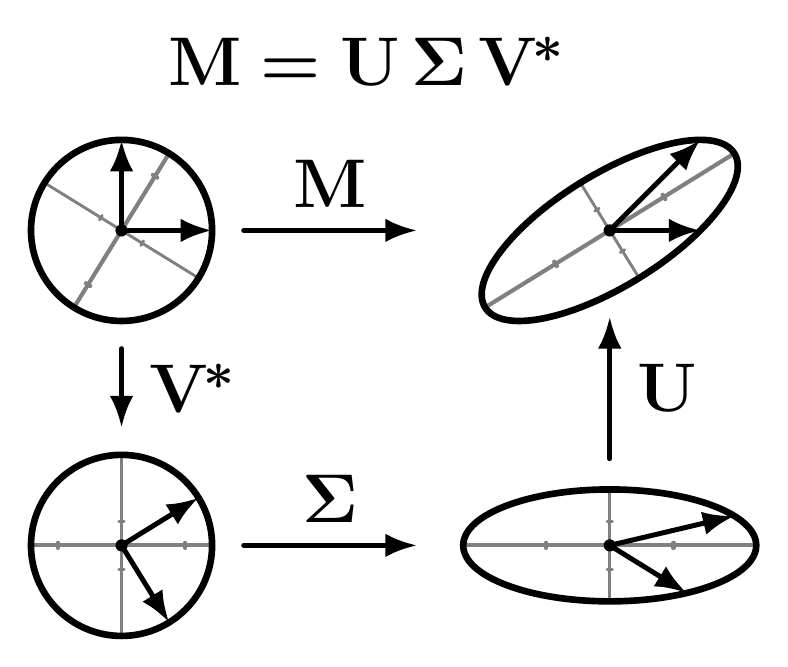
\begin{tikzpicture}[
  line cap=round,
  line join=round,
  >={Latex[length=4mm,width=3mm]},
  transform/.style={->, line width=1.7pt},
  boundary/.style={draw=black, line width=2.4pt},
  vec/.style={->, draw=black, line width=1.8pt},
  singularone/.style={draw=black!50, line width=1.50pt},
  singulartwo/.style={draw=black!50, line width=1.05pt},
  center/.style={fill=black},
  op/.style={font=\fontsize{28}{32}\selectfont}
]

% ------------------------------------------------------------------
% Exact parameters for
%
%       M = [ 1  1 ] = U Sigma V^*
%           [ 0  1 ]
%
% The singular values are phi and 1/phi. V^* rotates clockwise by
% alpha = atan(phi), while U rotates counterclockwise by
% beta = atan(1/phi).
% ------------------------------------------------------------------
\pgfmathsetmacro{\golden}{(1+sqrt(5))/2}
\pgfmathsetmacro{\invgolden}{1/\golden}
\pgfmathsetmacro{\alphaang}{atan(\golden)}
\pgfmathsetmacro{\betaang}{atan(1/\golden)}

\pgfmathsetmacro{\R}{1.15}
\pgfmathsetmacro{\major}{\golden*\R}
\pgfmathsetmacro{\minor}{\invgolden*\R}

% Tick placement.  The two families keep their different line weights, and the
% ticks are placed at distances from the center proportional to the associated
% singular values: d_i = tickbase * sigma_i.
\pgfmathsetmacro{\tickbase}{0.50}
\pgfmathsetmacro{\tickonepos}{\tickbase*\golden}
\pgfmathsetmacro{\ticktwopos}{\tickbase*\invgolden}
\pgfmathsetmacro{\tickhalf}{0.033}

% Panel centers.
\coordinate (A) at (0,4.0);   % input disk
\coordinate (B) at (0,0);     % after V^*
\coordinate (C) at (6.2,0);   % after Sigma V^*
\coordinate (D) at (6.2,4.0); % after U Sigma V^* = M

% ------------------------------------------------------------------
% Main equation.
% The equal sign and adjoint star are deliberately heavier for printing.
% ------------------------------------------------------------------
\node[font=\fontsize{38}{44}\selectfont] at (3.1,6.15)
  {$\mat{M}\thickeq\mat{U}\,\mat{\Sigma}\,\mat{V}\adj$};

% ------------------------------------------------------------------
% A: input unit disk.
%
% The gray diameters are the right singular directions v_1 and v_2,
% i.e. the columns of V. Since V = R(alpha), these axes are rotated by alpha.
% Their different line weights are retained, and each family also gets
% symmetric perpendicular ticks. The heavy arrows e_1,e_2 are retained as
% reference vectors whose complete images are followed around the diagram.
% ------------------------------------------------------------------
\begin{scope}[shift={(A)}]
  \begin{scope}[rotate=\alphaang]
    \singulardia{singularone}{\R}{\tickonepos}{\tickhalf}
    \begin{scope}[rotate=90]
      \singulardia{singulartwo}{\R}{\ticktwopos}{\tickhalf}
    \end{scope}
  \end{scope}

  \draw[boundary] (0,0) circle[radius=\R];
  \draw[vec] (0,0) -- (\R,0);
  \draw[vec] (0,0) -- (0,\R);
  \fill[center] (0,0) circle[radius=2.2pt];
\end{scope}

% ------------------------------------------------------------------
% B: after V^*.
%
% V^* maps the right singular directions to the coordinate axes, while the
% disk itself remains a disk because V^* is orthogonal.
% ------------------------------------------------------------------
\begin{scope}[shift={(B)}]
  \singulardia{singularone}{\R}{\tickonepos}{\tickhalf}
  \begin{scope}[rotate=90]
    \singulardia{singulartwo}{\R}{\ticktwopos}{\tickhalf}
  \end{scope}

  \draw[boundary] (0,0) circle[radius=\R];

  % V^* e1
  \draw[vec] (0,0) --
    ({\R*cos(\alphaang)},{-\R*sin(\alphaang)});

  % V^* e2
  \draw[vec] (0,0) --
    ({\R*sin(\alphaang)},{\R*cos(\alphaang)});

  \fill[center] (0,0) circle[radius=2.2pt];
\end{scope}

% ------------------------------------------------------------------
% C: after Sigma V^*.
%
% Sigma scales the two singular axes independently. The gray lines remain the
% principal axes of the ellipse. Tick positions continue to encode the two
% singular-value families while avoiding a misleading rescaling of line weight.
% ------------------------------------------------------------------
\begin{scope}[shift={(C)}]
  \singulardia{singularone}{\major}{\tickonepos}{\tickhalf}
  \begin{scope}[rotate=90]
    \singulardia{singulartwo}{\minor}{\ticktwopos}{\tickhalf}
  \end{scope}

  \draw[boundary] (0,0) ellipse[x radius=\major,y radius=\minor];

  % Sigma V^* e1
  \pgfmathsetmacro{\cOneX}{\R*\golden*cos(\alphaang)}
  \pgfmathsetmacro{\cOneY}{-\R*\invgolden*sin(\alphaang)}
  \draw[vec] (0,0) -- (\cOneX,\cOneY);

  % Sigma V^* e2
  \pgfmathsetmacro{\cTwoX}{\R*\golden*sin(\alphaang)}
  \pgfmathsetmacro{\cTwoY}{\R*\invgolden*cos(\alphaang)}
  \draw[vec] (0,0) -- (\cTwoX,\cTwoY);

  \fill[center] (0,0) circle[radius=2.2pt];
\end{scope}

% ------------------------------------------------------------------
% D: after U.
%
% U rotates the principal directions rigidly by beta. The heavy arrows are
% M e1=(1,0) and M e2=(1,1), exact for the chosen shear.
% ------------------------------------------------------------------
\begin{scope}[shift={(D)}]
  \begin{scope}[rotate=\betaang]
    \singulardia{singularone}{\major}{\tickonepos}{\tickhalf}
    \begin{scope}[rotate=90]
      \singulardia{singulartwo}{\minor}{\ticktwopos}{\tickhalf}
    \end{scope}
    \draw[boundary] (0,0) ellipse[x radius=\major,y radius=\minor];
  \end{scope}

  \draw[vec] (0,0) -- (\R,0);
  \draw[vec] (0,0) -- (\R,\R);
  \fill[center] (0,0) circle[radius=2.2pt];
\end{scope}

% ------------------------------------------------------------------
% Transformation arrows.
% ------------------------------------------------------------------
\draw[transform] ($(A)+(1.55,0)$) -- ($(D)+(-2.45,0)$)
  node[midway, above=4pt, op] {$\mat{M}$};

\draw[transform] ($(A)+(0,-1.50)$) -- ($(B)+(0,1.50)$)
  node[midway, right=6pt, op] {$\mat{V}\adj$};

\draw[transform] ($(B)+(1.55,0)$) -- ($(C)+(-2.45,0)$)
  node[midway, above=4pt, op] {$\mat{\Sigma}$};

\draw[transform] ($(C)+(0,1.10)$) -- ($(D)+(0,-1.10)$)
  node[midway, right=6pt, op] {$\mat{U}$};

\end{tikzpicture}

\end{document}

